\section{Temporal Metadata Model} \label{section:temporal}

In this section, we extend our metadata model with a temporal dimension that
enables the applications in Section~\ref{section:motivation}. To do this effectively, we first
discuss our notions of \emph{time} and how to mitigate discrepancies between client and server.
We then examine established temporal data models such as the Bitemporal Conceptual Data Model (BCDM).
Because most research into temporal data models has been conerned with relational or spatial models,
these models are more complicated than needed for a simple EAV table.

\begin{itemize}
\item then start talking about temporal query languages?
\item temporal query language tquel~\cite{snodgrass1987temporal}
\item tsql2~\cite{snodgrass2012tsql2}
\item tquery~\cite{kahn1991tquery}
\item differentiate from continuous query languages like CQL~\cite{arasu2006cql}
\end{itemize}

\subsection{What is Time?}

There are two flavors of time that temporal database must deal with:
\emph{valid time} and \emph{transaction time}~\cite{jensen1999temporal}\cite{jensen1996semantics}. 

\textbf{Valid time} is the extent for which a given \emph{fact} is true. For
our model, a fact is the association of a key-value pair with a stream,
changing the value associated with a stream's key, or removing a key-value pair
from a stream's metadata. Valid time is expressed in terms of real-world time
and is how metadata facts are aligned with timeseries data, which is stored
using real-world time. Because valid time is the coordinating aspect across the
two databases (timeseries and metadata), it is also the point of interaction
for consumers of data.

A fact's valid time can be qualified either by a single time (``start'') or by
a duration (``start'' and ``end''). Duration-based facts are used in most of
the established relational models (I believe because they make temporal joins
easier to reason about).  The use of a start-time lends itself to diff-based
storage, where facts for each \texttt{<uuid, key>} pair are considered valid
until a new fact is written for the same \texttt{<uuid, key>} pair. This also
removes the need to invalidate past facts, which is a drawback of the
bitemporal model (BCDM).

\textbf{Transaction time} is a logical timestamp that represents when a fact
takes place in relation to other facts. In a temporal database where all
entries are made at the current time, transaction time can be conflated with
valid time, but if the database allows retroactive inserts, then these two
times must be separate. In our demo implementation, transaction time is made
implicit through the use of transactions on the underlying database. Unlike
valid times, which maybe added in the past, transaction times are strictly
monotonic.

A temporal database must decide whether or not to make these timestamps
explicit in the representation and query interface.  While these two views of
time are orthogonal~\cite{snodgrass1986temporal}, some databases such as
POSTGRES~\cite{stonebraker1990implementation} conflate the two into transaction
time and only maintain a history of changes so far as to resolve concurrent
transactions. Transaction times are useful for ordering incoming operations,
but do not need to be factored into the query model. Thus, our model makes
valid timestamps explicit in the storage and retrieval of facts, but
transaction times are kept internal to the DBMS.

\if 0
have a figure here? start-time vs duration time?
\fi

\subsection{Established Temporal Data Models}

The \textbf{Temporally Oriented Data Model}~\cite{ariav1986temporally} (TODM)
stores temporal data along the 3 dimensions of objects, attributes and
time. TODM makes an assumption of temporal isomorphism, that is, ``there is a tight
correspondence between the database and the temporally concurrent reality it is
aimed to capture.''\cite{ariav1986temporally}. This seems to preclude
insertions into the past, but TODM does use this restriction to avoid
penalizing queries interested in the most current version of an object, which
is a design goal for our approach as well. We wish to preserve the 3-dimensioanl
relation of object (UUID), attribute (key-value) and time, but with valid
and transactional times decoupled.

\textbf{The Generalized Model for a Relational Temporal Database}~\cite{gadia1988generalized} proposes a two-dimensional
model that preserves both real world (valid) and transactional timestamps of a
tuple, but is directed towards fully relational representations of data.  The
disadvantage of the model -- for a fully general temporal relational database
-- is that it cannot express valid times that occur after the transaction
time\footnote{This is not a feature that our model needs to support}.

\todo{think abou this next part}
Generalized Model for a Relational Temporal
Database~\cite{gadia1988generalized} makes the observation that ``intervals are
not closed under union, intersection and complementation, and thus are not
adequate to model natural language queries involving `or', `and' and `not'.''

The \textbf{Historical Database Management System} (HDBMS)
model~\cite{sarda1990extensions} uses an extended relational model, in which
all tuples are stored normally but with the addition of interval timestamps.
The associated query language, HSQL, uses this extension for operations such as
time-based joins. 

A point of major simplification in our model is that we do not need to directly
support joins based on time, meaning we can retain all of our relational
algebra, and use simple qualifiers on time instants and extents to further
restrict the evaluations of their associated predicates.

\cite{jensen1994unifying} proposes the \textbf{Bitemporal conceptual data
model} (BCDM), which stores relations with 4 additional columns: valid
start/end time and transaction start/end time. However, due to the complexity
(and completeness) of the model, \cite{jensen1999temporal} asserts that there
is much work to be done on evaluating the performance of the extended
relational algebra as well as how to efficiently implement a compliant
database.
\todo{bcdm has to be updated at every tick to be correct? This is very slow!}

%\begin{itemize}
%%\item BCDM bitemporal conceptual data model: only captures when facts are valid in reality and when stored in database~\cite{jensen1996semantics}\cite{jensen1994unifying}
%\item incremental relational temporal model: \cite{jensen1991incremental}
%\item relational algebra accounts for transaction time, evolution of contents as well as schema~\cite{mckenzie1990schema}
%\end{itemize}

\subsection{EAV-Based Temporal Data Model}

We choose a natural extension of the entity-attribute-value model described in Section~\ref{section:model}.
Because of our restrictions on the usual temporal models -- not needing to support joins on time or fully
general relational algebra, and only supporting queries on valid time -- our temporal extension can remain
simple.

\textbf{Construction.} we extend the entity-attribute-value model with a 4th dimension representing the initial
valid time of a fact. Each fact (row) can take one of two forms: an insertion of \texttt{<uuid, key, value, timestamp>}
or a deletion with \texttt{<uuid, key, NULL, timestamp>}. For an example fact $<u_0, k_0, v_0, t_0>$, the \texttt{value} $v_0$ is valid (true) for the tuple $<u_0, k_0>$
with real-world \texttt{timestamp} $t_0$ starting at time $t_0$ and extending to the current time or until another
tuple with $<u_0, k_0>$ and real-world \texttt{timestamp} $t_1$ is inserted with $t_1 > t_0$. This diff-based approach
to storing persistent records makes it simple to compute the start/end valid times explicit in other temporal models.
Queries on the state of the database at time $t$ can be performed by ``searching'' backwards in time for 
records with timestamp $\leq t_0$ that match the provided relational predicate.

\if 0
What about writing into the past? inserts/deletions are easy because they are all just to the end of the log, but
we can run a garbage collection process that sorts them. If we use a SQL table, our generated SQL queries should
be able to avoid detecing duplicates in the result set, so no blocking needs to happen on running the log reordering
\fi

An illustration of this structure can be seen in Figure~\ref{figure:temporaleavexample} and Table~\ref{table:temporaleavexample}.

\begin{figure}
\centering
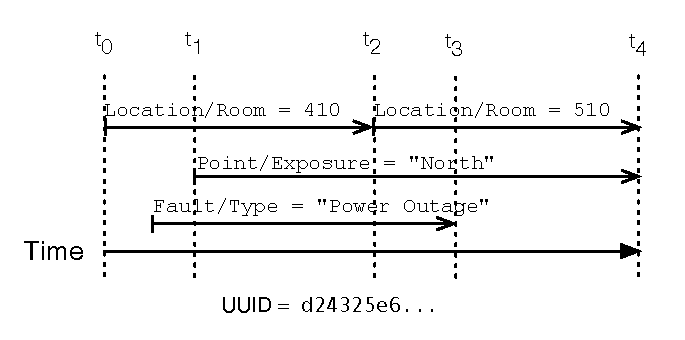
\includegraphics[width=.9\linewidth]{figs/time.pdf}
\caption{Visualization of the temporal EAV model in Table~\ref{table:temporaleavexample}}
\label{figure:temporaleavexample}
\end{figure}

\begin{table}
\centering
\begin{tabular}{|l|c|c|c|}
\hline
\textbf{UUID} & \textbf{Key} & \textbf{Value} & \textbf{Valid Time} \\
\hline
\end{tabular}
\caption{Tabular representaion of the temporal entity-attribute-value model}
\label{table:temporaleavexample}
\end{table}

\textbf{Where does time come from?}

Both our non-temporal (Figure~\ref{fig:nontemporalgrammar}) and temporal (Figure~\ref{fig:temporalgrammar}) query languages
support queries across two databases (timeseries and metadata). In designing the temporal model, we must account for
whose notion of time (client's or server's) is used for the valid time.

\if 0
clients need to be able to query each others streams
    - suggests server time
clients want to write into the past
    - suggests client time
    - maybe client can compute the real timestamp?
        client reports its current time and the diff to the time it wants to write at.
        server then shifts this up or down depending on what its current time is.
        This doesn't really account for time stretching?
    - clients write into past infrequently, so its okay to have this coordination be more expensive
optimize for common case: clients writing to current form of document -- just a log append
\fi
\if 0
THIS IS NOT NEW: find cites!
We choose a natural extension of the non-temporal entity-attribute-valuel model.
We track valid time, but use transactional time for logical ordering of queries/insertions
extend EAV table with 4th column for time
Insertions can occur with any valid time <= current time
We extend the query language with syntax to support qualifying the usual
relational predicates with time. 
\fi

\subsection{Proposed Temporal Query Language}

\if 0
First, lets establish a model for expressiveness: how do we know we've "covered" the space?

Want a diagram with our expressiveness timeline, with two streams, representing two attributes. We
have the usual one dimensional aspects we want to cover, but also draw a box/tetris shape over
the two streams at once to emphasize that we want to be able to cover across relations *and* across
time in the same query.
\fi

Figure~\ref{fig:temporalgrammar} contains a simplified grammar of our proposed temporal query language.

\setlength{\grammarindent}{8em}
\setlength{\grammarparsep}{4pt}
\begin{figure}
\centering
\begin{grammar}
<query> := `select' <selectClause> `where' <whereClause>

<selectClause> := <selectTerm>
\alt <selectTerm> `,' <selectClause>

<selectTerm> := <selectTermValue>
\alt `FIRST' <selectTermValue>
\alt `LAST' <selectTermValue>
\alt `ALL' <selectTermValue>
\alt <selectTermValue> `AT' <time>
\alt <selectTermValue> `IAFTER' <time>
\alt <selectTermValue> `IBEFORE' <time>
\alt <selectTermValue> `AFTER' <time>
\alt <selectTermValue> `BEFORE' <time>
\alt <selectTermValue> `IN' `(' <time> `,' <time> `)'

<selectTermValue> := <lvalue>
\alt `*'
\alt `DISTINCT' <lvalue>
\alt `DATA IN' `(' <time> `,' <time> `)'
\alt `DATA BEFORE' <time>
\alt `DATA AFTER' <time>

<whereClause> := <whereTerm> `AND' <whereClause>
\alt <whereTerm> `OR' <whereClause>
\alt `NOT' <whereClause>
\alt `(' <whereClause> `)'
\alt <whereTerm>

<whereTerm> := <predicate>
\alt <predicate> <temporalPredicate>

<predicate> := <lvalue> `LIKE' <rvalue>
\alt <lvalue> `=' <rvalue>
\alt <lvalue> `!=' <rvalue>
\alt `HAS' <lvalue>

<temporalPredicate> := `HAPPENS IN' `(' <time> `,' <time> `)'
\alt `HAPPENS BEFORE' <time>
\alt `HAPPENS AFTER' <time>
\alt `AT' <time>
\alt `FOR' `(' <time> `,' <time> `)'

<rvalue> := <string>
\alt <number>
\alt <regex>
\alt <uuid>

<lvalue> := <string>
\end{grammar}
\caption{Simplified grammar for the \emph{temporal} query language over timeseries and metadata}
\label{fig:temporalgrammar}
\end{figure}

%[39, 52, 53, 74]

%\begin{itemize}
%\item Discuss current tmporal data models
%    \begin{itemize}
%    \item TODO: make this list
%    \item OURS: how to augment with time: add column to EAV
%    \end{itemize}
%\item discuss sql vs nosql for demo implementation?
%    \begin{itemize}
%    \item SQL more suited for diffs?
%    \item NoSQL more suited for replication?
%    \end{itemize}
%\end{itemize}
%
Some related work:
\begin{itemize}
\item $<tt, vt>$ (timestamp, validtime) for temporal data~\cite{jensen1999temporal},
also stratum vs integrated approaches for implementing temporal databases
\item extending relational algebra for temporal data?~\cite{lorentzos1988extending}
\item list of temporal terms~\cite{dyreson1994consensus}
\end{itemize}
